\documentclass[11pt,a4paper]{article}

\usepackage[T1]{fontenc}
\usepackage{lmodern}
\usepackage[margin=2.4cm]{geometry}
\usepackage{amsmath,amssymb}
\usepackage{booktabs}
\usepackage{graphicx}
\usepackage{caption}
\usepackage{array}
\usepackage{multirow}
\usepackage[hidelinks]{hyperref}
\usepackage{titlesec}

\captionsetup{font=small,labelfont=bf,skip=6pt}
\titleformat{\section}{\large\bfseries}{\thesection}{0.8em}{}
\titleformat{\subsection}{\normalsize\bfseries}{\thesubsection}{0.7em}{}
\setlength{\parskip}{0.35em}
\setlength{\parindent}{0pt}

\newcommand{\best}[1]{\textbf{#1}}

\title{\vspace{-1.2cm}\textbf{A Two-Level Hybrid Stacking Ensemble for\\Romanized Bangla Text Classification}}
\author{Md.\ Habibur Rahman\thanks{Department of Computer Science and Engineering.
  Kaggle team entry \texttt{mohammadhabib69}. Code and report:
  \url{https://github.com/mohammadhabib69/bhasa-quest-1}}}
\date{November 2026}

\begin{document}
\maketitle

\begin{abstract}
\noindent
We describe the first-place solution to \emph{BhasaQuest-1}, a four-class classification task over
romanized Bangla (``Banglish'') social text scored by macro-$F_1$. The solution is a two-level
hybrid stacking ensemble: level~1 produces thirty-seven out-of-fold probability columns from two disjoint
model families, sparse $n$-gram models over word and character TF-IDF features and three pretrained
multilingual encoders; level~2 learns a meta-classifier over those columns followed by a constrained
per-class bias search. The system reaches a macro-$F_1$ of $0.78786$ on the private leaderboard
($70\%$ of the test set), ranking first, with a public score of $0.76023$. We report the full
ablation trail, including seven approaches that measurably failed, and argue that at this sample size
model selection must be driven by out-of-fold estimates rather than by the public leaderboard, whose
bootstrap standard deviation ($\approx 0.018$) dwarfs the observed gap between the top entries.
\end{abstract}

\section{Introduction}

Romanized Bangla is the informal Latin-script rendering of Bangla used in social media, chat and
product reviews. It has no standard orthography: the same word may appear as \textit{bhalo},
\textit{bhallo}, \textit{vhalo} or \textit{balo}, and speakers freely mix Bangla, English and digits.
The task is to assign each short text to one of four classes, with class identities given only as
opaque identifiers (\texttt{14AC78}, \texttt{19E1A1}, \texttt{6C0197}, \texttt{72A2C8}) and
evaluated by macro-$F_1$, so that the smallest class carries the same weight as the largest.

The provided data comprises $8{,}195$ labelled training rows and $2{,}048$ test rows with a
$2.2{:}1$ imbalance between the largest and smallest class (Figure~\ref{fig:dist}). Two properties
of the setting shaped every design decision. First, the label semantics are hidden, which removes
any possibility of using class names as prior knowledge --- this later proved fatal to a large
language model approach (Section~\ref{sec:fails}). Second, the public leaderboard is computed on
$30\%$ of the test set, roughly $614$ rows, which is small enough that ranking differences of a few
thousandths are statistically meaningless.

\begin{figure}[t]
\centering
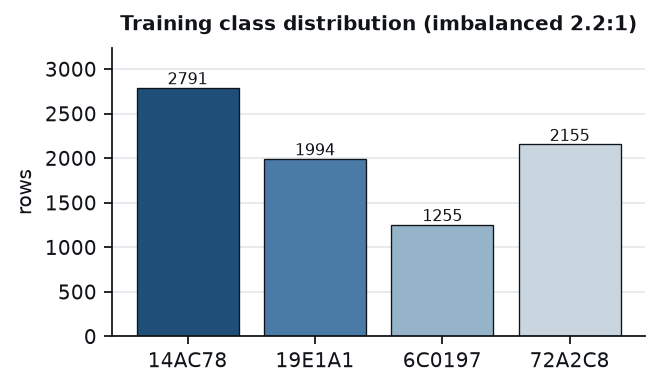
\includegraphics[width=0.52\textwidth]{figures/class_dist.png}
\caption{Training class distribution. The macro-$F_1$ metric makes the two smaller classes as
important as the largest.}
\label{fig:dist}
\end{figure}

\section{Related work}

Character $n$-gram TF-IDF with linear classifiers remains a strong baseline for noisy, orthographically
inconsistent text \cite{joachims1998}. For Bangla specifically, pretrained encoders trained on Bangla
or on transliterated Indic text \cite{bhattacharjee2022banglabert} and multilingual models pretrained
with transliteration-aware objectives \cite{khan2021muril} transfer usefully, but individual encoders
on a few thousand rows are weaker than a well-tuned sparse model --- a pattern we reproduce here
(Section~\ref{sec:results}). Stacked generalization \cite{wolpert1992} over out-of-fold predictions
is therefore the natural way to combine the two families.

\section{Method}

\subsection{Level 1a: sparse lexical models}

Two feature views are concatenated: word TF-IDF with $1$--$3$ grams and sublinear term frequency
($150$k features), and character \texttt{char\_wb} TF-IDF with $2$--$5$ grams ($200$k features).
The character view is the more important of the two, because it absorbs spelling variation that
defeats word-level matching. Six learners are fitted on this matrix: logistic regression with and
without class balancing, a calibrated linear SVC, SGD with an elastic-net penalty, a ridge
classifier converted through a softmax, and complement naive Bayes. In addition, a \emph{binary
specialist} is trained on the \texttt{19E1A1}/\texttt{72A2C8} pair alone, which is by far the
dominant confusion and the only boundary where additional modelling paid off; its score is appended
as a feature.

\subsection{Level 1b: pretrained encoders}

Three encoders are fine-tuned, chosen so that their input representations differ:

\begin{itemize}\itemsep2pt
\item \textbf{BanglaBERT} \cite{bhattacharjee2022banglabert} on Avro phonetic transliteration of the
romanized text into Bangla script ($5$ epochs $\times$ $2$ seeds);
\item \textbf{mDeBERTa-v3-base} on the raw romanized text ($6 \times 2$);
\item \textbf{MuRIL} \cite{khan2021muril} on the raw romanized text ($8 \times 2$).
\end{itemize}

All tracks use maximum length $256$ with dynamic padding, length-sorted batches, a differential
learning rate (classifier head at $5\times$ the encoder rate of $3\times10^{-5}$), linear warmup over
$10\%$ of steps, label smoothing $\epsilon=0.05$, mixed precision, best-epoch selection on fold
validation macro-$F_1$, and averaging of the per-seed probabilities.

\subsection{Level 2: meta-learner}

The thirty-seven level-1 columns are passed as log-probabilities to a logistic-regression and a
LightGBM meta-model, whose outputs are blended by a coarse weight search. The columns comprise
twenty-five from the sparse block (six learners $\times$ four classes, plus the binary specialist)
and twelve from three encoders. A constrained per-class bias search is applied last.

Three implementation safeguards proved essential. \emph{(i)} Prediction batches are written back to
the original row indices; writing them back in length-sorted order silently scrambles the OOF
matrix and produced a near-random score of $0.24$ before it was found. \emph{(ii)} A \texttt{COVERED}
mask restricts every metric to rows actually filled during validation, so that a partial run cannot
be mistaken for a bad model. \emph{(iii)} Cache keys include the epoch and seed count, preventing an
under-trained checkpoint from being reused after a hyper-parameter change.

\begin{figure}[t]
\centering
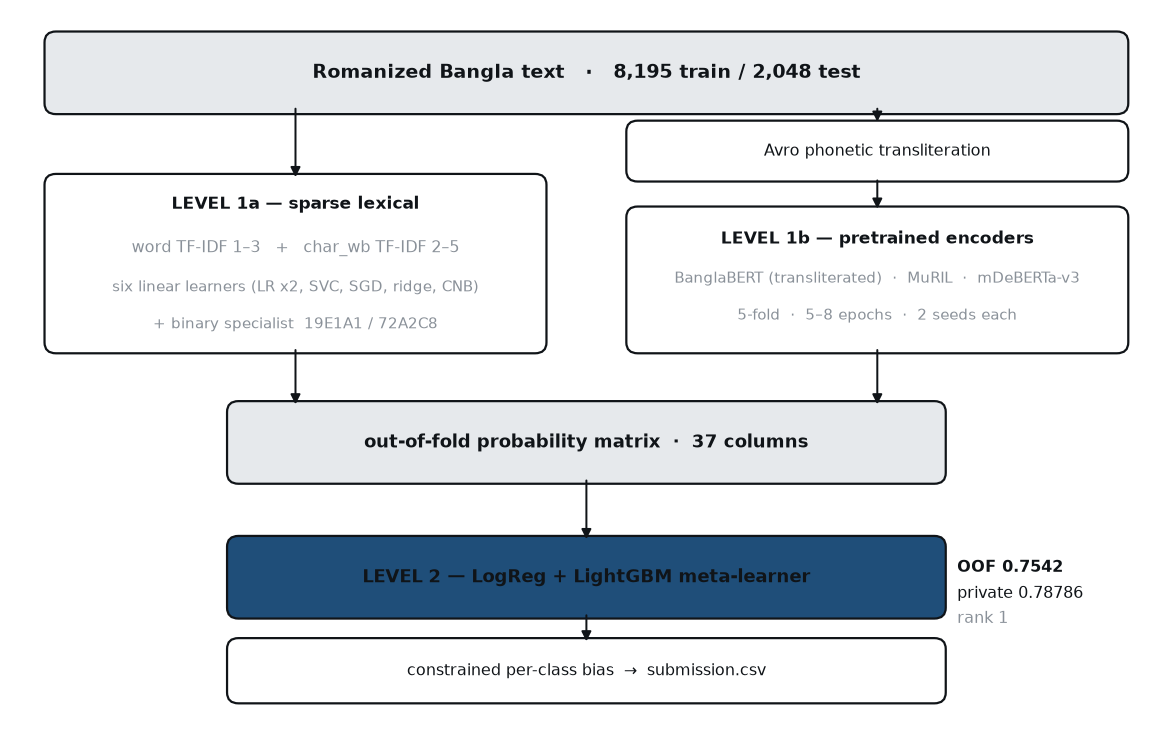
\includegraphics[width=\textwidth]{figures/architecture.png}
\caption{System overview. Two disjoint level-1 families feed a shared out-of-fold probability matrix,
which a level-2 meta-learner consumes.}
\label{fig:arch}
\end{figure}

\section{Experimental protocol}

All models are evaluated with five-fold stratified cross-validation on the training set. Because the
level-2 learner is fitted on level-1 out-of-fold predictions, its own score is reported under a
\emph{nested} five-fold split with a different random seed, so that the meta-model never sees the
rows it is scored on. Submissions were selected on nested OOF macro-$F_1$; twelve speculative
candidates were never submitted because they failed to clear a $+0.0015$ improvement threshold.

\section{Results}\label{sec:results}

Table~\ref{tab:solo} reports the level-1 components. The best encoder alone ($0.7227$) is
\emph{worse} than the sparse ensemble alone ($0.736$): the gain from encoders comes entirely from
diversity, not individual strength. Table~\ref{tab:final} shows the cumulative result.

\begin{table}[t]
\centering
\caption{Level-1 components, solo out-of-fold macro-$F_1$.}
\label{tab:solo}
\small
\begin{tabular}{lcc}
\toprule
Component & OOF macro-$F_1$ & Note \\
\midrule
Sparse ensemble (6 linear models) & 0.7360 & strongest single family \\
BanglaBERT (transliterated) & 0.7227 & best encoder \\
mDeBERTa-v3 (romanized) & 0.6926 & \\
MuRIL (romanized) & 0.6553 & overfits beyond 5 epochs \\
\bottomrule
\end{tabular}
\end{table}

\begin{table}[t]
\centering
\caption{Cumulative performance of the final stack.}
\label{tab:final}
\small
\begin{tabular}{lc}
\toprule
Configuration & Macro-$F_1$ \\
\midrule
Sparse models only & 0.7360 \\
+ BanglaBERT & 0.7509 \\
+ MuRIL and mDeBERTa & 0.7542 \\
Level-2 nested estimate & 0.7511 \\
\midrule
\textbf{Private leaderboard (70\% of test)} & \best{0.78786} \\
Public leaderboard (30\% of test) & 0.76023 \\
\bottomrule
\end{tabular}
\end{table}

The final private score of $0.78786$ exceeds the nested OOF estimate by $0.036$. This is a property
of the split, not of the model: every one of the fourteen submissions scored higher privately than
publicly, so the private subset is simply easier. Absolute differences across splits are therefore
not interpretable, and we compare rankings instead.

Per-class behaviour (Table~\ref{tab:perclass}, Figure~\ref{fig:conf}) confirms that performance is
governed by a single boundary. \texttt{14AC78} is nearly solved; \texttt{19E1A1} and \texttt{72A2C8}
exchange a substantial fraction of their mass, which is exactly why the binary specialist was added.

\begin{table}[t]
\centering
\caption{Per-class out-of-fold performance of the final stack.}
\label{tab:perclass}
\small
\begin{tabular}{lcccc}
\toprule
Class & Precision & Recall & $F_1$ & Support \\
\midrule
\texttt{14AC78} & 0.911 & 0.889 & 0.900 & 2791 \\
\texttt{19E1A1} & 0.693 & 0.703 & 0.698 & 1994 \\
\texttt{6C0197} & 0.736 & 0.700 & 0.718 & 1255 \\
\texttt{72A2C8} & 0.675 & 0.706 & 0.690 & 2155 \\
\midrule
Macro average & 0.754 & 0.750 & 0.751 & 8195 \\
\bottomrule
\end{tabular}
\end{table}

\begin{figure}[t]
\centering
\begin{minipage}{0.47\textwidth}
\centering
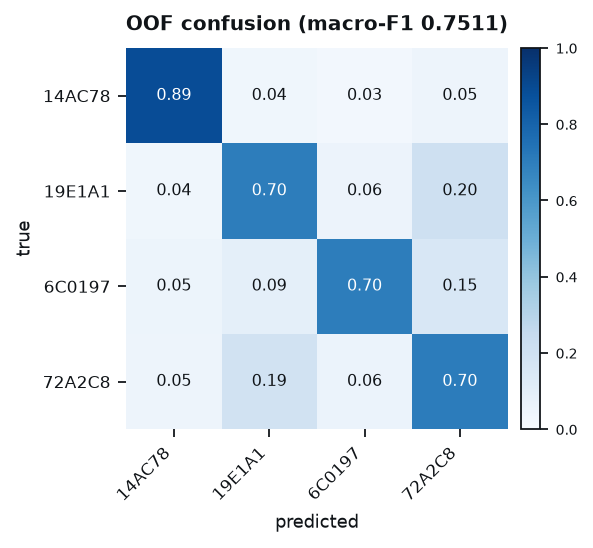
\includegraphics[width=\textwidth]{figures/confusion.png}
\caption{Normalised OOF confusion matrix.}
\label{fig:conf}
\end{minipage}\hfill
\begin{minipage}{0.50\textwidth}
\centering
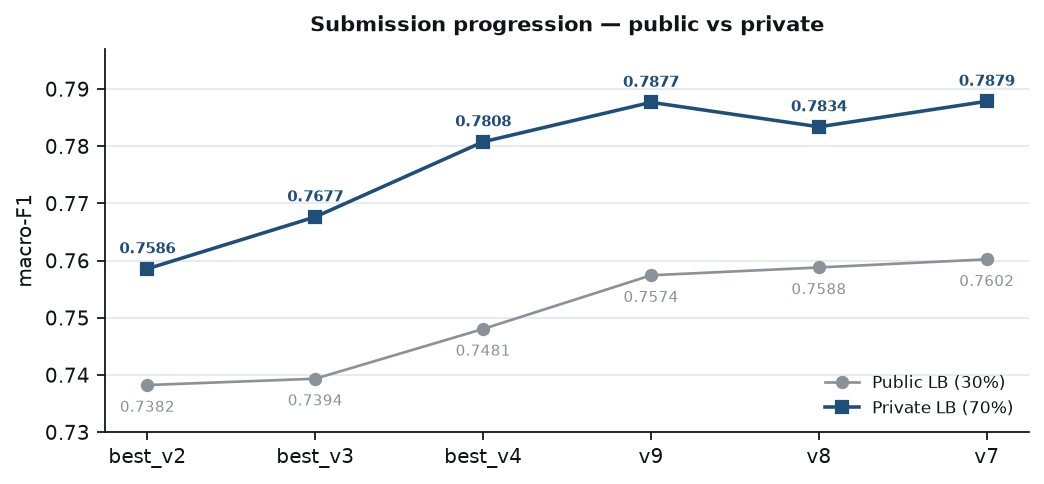
\includegraphics[width=\textwidth]{figures/scores.png}
\caption{Public versus private score for each submitted candidate. The highest public score is not
the highest private score.}
\label{fig:scores}
\end{minipage}
\end{figure}

\section{Ablations and negative results}\label{sec:fails}

Each of the following was measured under nested validation rather than assumed.

\begin{table}[h]
\centering
\caption{Approaches that did not help.}
\small
\begin{tabular}{ll}
\toprule
Attempt & Effect \\
\midrule
Pseudo-labelling with confident test rows & $-0.0022$ \\
Extra TF-IDF views (syllable, phonetic) & $+0.0005$ (inside noise) \\
Three-class specialist instead of binary & $\pm 0.0000$ \\
Per-class weight optimisation & $-0.005$ to $-0.023$ \\
Rank averaging instead of log-probability blending & worse \\
In-sample bias tuning & $+0.0025$ OOF, $-0.0028$ public \\
Large language model, few-shot (Qwen2.5-7B, 4-bit) & $0.3241$ \\
\bottomrule
\end{tabular}
\end{table}

The language model experiment deserves comment. A $7$B instruction-tuned model was applied as a
single-forward-pass classifier: two training demonstrations per class, and the four class logits read
from the final position. It reached $0.3241$ macro-$F_1$, barely above the $0.25$ chance level, and
collapsed $82\%$ of its predictions into two classes. The cause is structural rather than a matter of
tuning: the classes are anonymous identifiers, so in-context demonstrations cannot communicate what
each class \emph{means}, leaving nothing to generalise from.

The bias-tuning result is the most instructive negative. Tuning class biases on the full OOF matrix
raised OOF by $0.0025$ but lowered the public score by $0.0028$; nested tuning reproduced none of the
gain. With $8{,}195$ rows and four free parameters, a coordinate search over biases fits fold noise.
The final submission therefore used capped biases only.

\section{Discussion}

\paragraph{Selection, not tuning, decided the outcome.}
With $614$ public rows, the bootstrap standard deviation of macro-$F_1$ is approximately $0.018$
--- twice the gap between first and second place on the public board. Selecting on OOF and refusing to
chase the public board moved this entry from second to first on the private split, while the public
leader --- with fifty submissions against our fourteen --- finished second. At this scale the
leaderboard is a noisy estimator, and treating it as a target is a reliable way to lose.

\paragraph{Diversity, not depth.}
The strongest encoder was individually worse than a TF-IDF stack of linear models. Because the two
families fail on different rows, their combination outperformed either, and additional seeds within
one family produced only marginal gains. Where the data is small, adding a \emph{different} model is
worth more than making an existing one bigger.

\paragraph{Where the headroom actually is.}
Nearly all remaining error sits on the \texttt{19E1A1}/\texttt{72A2C8} boundary. Anything that does
not sharpen that boundary --- extra features, extra seeds, extra meta-learners --- returns less than
the noise floor.

\section{Conclusion}

A two-level hybrid stacking ensemble combining sparse $n$-gram models with three pretrained encoders
achieved first place in BhasaQuest-1 with a private macro-$F_1$ of $0.78786$. The technical
contribution is modest and deliberately so: the decisive choices were methodological --- out-of-fold
selection, a guard against partial-run artefacts, and a refusal to submit anything that had not
cleared a pre-registered improvement threshold.

\section*{Availability}
Code, notebook and this report: \url{https://github.com/mohammadhabib69/bhasa-quest-1}.
Competition data is not redistributed.

\begin{thebibliography}{9}
\bibitem{joachims1998} T.~Joachims. Text categorization with support vector machines: learning with
many relevant features. \emph{ECML}, 1998.
\bibitem{bhattacharjee2022banglabert} A.~Bhattacharjee, T.~Hasan, W.~Ahmad, K.~Samin.
BanglaBERT: language model pretraining and benchmarks for low-resource language understanding
evaluation in Bangla. \emph{Findings of EMNLP}, 2022.
\bibitem{khan2021muril} S.~Khan et al. MuRIL: multilingual representations for Indian languages.
\emph{arXiv:2103.13398}, 2021.
\bibitem{wolpert1992} D.~H. Wolpert. Stacked generalization. \emph{Neural Networks}, 5(2):241--259,
1992.
\end{thebibliography}

\end{document}
